\documentclass[thesis.tex]{subfiles}

\begin{document}

Linked-cluster theorem,
\begin{equation}
  \ket{\Psi^{(1)}} = \sddiagram{MBPT_linked/MBPT_linked-figure0} + \sdiagram{MBPT_linked/MBPT_linked-figure1}
\end{equation}
\begin{align}
  \ket{\Psi^{(2)}} &= \sdiagram{MBPT_linked/MBPT_linked-figure2} + \sdiagram{MBPT_linked/MBPT_linked-figure3} + \sddiagram{MBPT_linked/MBPT_linked-figure4} + \sddiagram{MBPT_linked/MBPT_linked-figure5} \notag \\
  &+ \sddiagram{MBPT_linked/MBPT_linked-figure6} + \sddiagram{MBPT_linked/MBPT_linked-figure7} + \sddiagram{MBPT_linked/MBPT_linked-figure8} + \sddiagram{MBPT_linked/MBPT_linked-figure9} + \sddiagram{MBPT_linked/MBPT_linked-figure10} \notag \\
  &+ \sddiagram{MBPT_linked/MBPT_linked-figure11} + \sddiagram{MBPT_linked/MBPT_linked-figure12} + \sdiagram{MBPT_linked/MBPT_linked-figure13} + \sdiagram{MBPT_linked/MBPT_linked-figure14} + \sdiagram{MBPT_linked/MBPT_linked-figure15} \notag \\
  &+ \sdiagram{MBPT_linked/MBPT_linked-figure16} + \sdiagram{MBPT_linked/MBPT_linked-figure17} + \sdiagram{MBPT_linked/MBPT_linked-figure18} + \sdiagram{MBPT_linked/MBPT_linked-figure19} + \sdiagram{MBPT_linked/MBPT_linked-figure20}
\end{align}


Coupled cluster (CC) theory is based on expressing the $N$-particle correlated wave function $\corrket$ using the exponential ansatz,
\begin{align*}
  \corrket = e^{\hat{T}} \refket,
\end{align*}
where $\refket$ is the reference state as before.  The cluster operator $\Top \equiv \Top_{1} + \Top_{2} + \cdots + \Top_{N}$, is composed of $k$-particle $k$-hole excitation operators, $\Top_{k}$,
\begin{align} \label{eq:cc_amps}
  \hat{T}_{k} \equiv \left(\frac{1}{k!}\right)^2 \sum_{\substack{a_1 \ldots a_k \\ i_1 \ldots i_k}} \amp{a_1 \ldots a_k}{i_1 \ldots i_k}\normord{\hat{a}_{1}^\dagger \ldots \hat{a}_{k}^\dagger \hat{i}_{k}^{} \ldots \hat{i}_{1}^{}},
\end{align}
where the unknown matrix elements, $\amp{a_1 \ldots a_k}{i_1 \ldots i_k}$, are known as \textit{cluster amplitudes} \cite{SHAVITT2009}.

Using the CC ansatz, the Schr\"odinger equation,
\begin{align} \label{eq:cc_schrodeq}
  \Ham \E^{\Top} \refket = E \E^{\Top} \refket,
\end{align}
can be rewritten by left-multiplying by $\refbra \E^{-\Top}$ as,
\begin{align*}
  \refbra\EHam\refket = E,
\end{align*}
where we define a \textit{coupled cluster effective Hamiltonian},
\begin{align} \label{eq:cc_heff0}
  \EHam \equiv \E^{-\Top} \Ham \E^{\Top},
\end{align}
in which the wave operator, $\E^{\Top}$, acts as a similarity transform on the Hamiltonian in the same way that $\hat{U}(s)$ acts to transform the Hamiltonian in SRG methods.  An important difference, however, is that the wave operator in CC, which contains no de-excitations, is not unitary, and thus $\EHam$ is not Hermitian.

The effective Hamiltonian in Eq.\ \eqref{eq:cc_heff0} can be rewritten with commutators according to the Baker--Campbell--Hausdorff expansion as,
\begin{align*}
  \EHam = \Ham + [\Ham, \Top] + \frac{1}{2!} [[\Ham, \Top], \Top] + \frac{1}{3!} [[[\Ham, \Top], \Top], \Top] + \frac{1}{4!} [[[[\Ham, \Top], \Top], \Top], \Top],
\end{align*}
which terminates at four-nested commutators due to the two-body nature of the interaction.  Like with IM-SRG, this commutator expression ensures that CC is size-extensive and contains only connected terms.  In addition, because $\Top$ is an excitation operator, terms of the form $\Top\Ham$ are disconnected and thus vanish \cite{SHAVITT2009}.  Therefore the CC effective Hamiltonian can be further reduced to
\begin{align} \label{eq:cc_heff1}
  \EHam = \left(\Ham e^{\hat{T}}\right)_{\mathrm{c}},
\end{align}
where the subscript ``$\mathrm{c}$'' indicates that only connected terms are used.

In practice, the cluster operator $\Top$ must be truncated for calculations to be computationally feasible.  In this work, we use only single and double excitations,
\begin{align*}
  \Top = \Top_{1} + \Top_{2}.
\end{align*}
This is known as coupled cluster with singles and doubles (CCSD), with an asymptotic computational cost that scales like IM-SRG(2).  This truncation has been successfully applied to many problems in quantum chemistry \cite{BARTLETT2007291} and nuclear physics \cite{HAGEN2014096302}.  In addition, we also truncate the three-body effective Hamiltonian terms that are induced by the similarity transformation.  Fig.\ \ref{fig:diagrams-ccsd} shows the diagrammatic representation of Eq.\ \eqref{eq:cc_heff1} in CCSD.

\begin{figure}
  \includegraphics{fig-diagrams-ccsd.pdf}
  \caption{(Color online) Diagrammatic representation of $\bar{H}$ of Eq.\ \eqref{eq:cc_heff1}, excluding terms involving the one-body interaction $\hat{H}_1$ and first-order terms involving only the bare Hamiltonian. Open circles represent the excitation cluster operators $\hat{T}_1$ and $\hat{T}_2$, and filled circles represent the two-body interaction $\hat{H}_2$.  As before, the diagrams are implicitly antisymmetrized (Hugenholtz diagrams).  Lines connected to $\hat{T}$ are always directed upward because they represent an excitation operator while the directions of external lines connected to $\hat{H}_2$ are unconstrained. }
  \label{fig:diagrams-ccsd}
\end{figure}

The unknown cluster amplitudes in CCSD, $\amp{a}{i}$ and $\amp{ab}{ij}$, are calculated by left-multiplying Eq.\ \eqref{eq:cc_schrodeq} by $\statebra{a}{i} \E^{-\Top}$ and $\statebra{ab}{ij} \E^{-\Top}$, respectively,
\begin{align} \label{eq:ccsd1}
  \statebra{a}{i} \EHam \refket &= 0, \\
  \statebra{ab}{ij} \EHam \refket &= 0. \notag
\end{align}
After the Fock matrix has been diagonalized, the diagonal components of Eq.\ \eqref{eq:ccsd1} can be separated and, after expanding the exponent in Eq.\ \eqref{eq:cc_heff1}, the non-vanishing terms of the CCSD amplitude equations become,
\begin{gather} \label{eq:ccsd2}
  \statebra{a}{i} \left[ \Ham_{2} \left(\Top_{1} + \Top_{2} + \Top_{1}\Top_{2} + \frac{1}{2!} \Top_{1}^{2} + \frac{1}{3!} \Top_{1}^{3}\right) \right]_{\mathrm{c}} \refket = \Edenom{a}{i}\amp{a}{i} \\
  \statebra{ab}{ij} \left[ \Ham_{2} \left(1 + \hat{T}_1 + \hat{T}_2 + \frac{1}{2} \hat{T}_1^{2} + \hat{T}_1\hat{T}_2 + \frac{1}{2!} \hat{T}_2^{2} + \frac{1}{3!} \hat{T}_1^{3} + \frac{1}{2!} \hat{T}_1^{2} \hat{T}_2 + \frac{1}{4!} \hat{T}_1^{4}\right) \right]_{\mathrm{c}} \refket = \Edenom{ab}{ij}\amp{ab}{ij} \notag
\end{gather}
where $\Edenom{}{}$ are the M\o ller--Plesset denominators from Eq.\ \eqref{eq:moellerplessetdenominator}.  As usual, these non-linear equations are solved using an iterative procedure where the cluster amplitudes on the right-hand side of Eq.\ \eqref{eq:ccsd2} are updated by calculating the terms on the left-hand side until a fixed point is reached.  Like the HF iterative procedure, employing convergence acceleration techniques can reduce the number of CC iterations required.


\begin{equation}
  E\left( \Top, \Lop \right) = \refbra\Lop \E^{-\Top} \Ham \E^{\Top}\refket = \refbra\Lop \EHam\refket
\end{equation}
\begin{equation}
  \Lop \equiv \lamp{}{0} + \Lop_{1} + \Lop_{2} + \cdots + \Lop_{N}
\end{equation}
\begin{equation}
  \Lop_{k} \equiv \left(\frac{1}{k!}\right)^2 \sum_{\substack{a_1 \ldots a_k \\ i_1 \ldots i_k}} \lamp{i_1 \ldots i_k}{a_1 \ldots a_k}\normord{\hat{i}_{1}^\dagger \ldots \hat{i}_{k}^\dagger \hat{a}_{k}^{} \ldots \hat{a}_{1}^{}},
\end{equation}
\begin{align}
  \refbra \Lop\left[ \EHam, \normord{\hat{a}^{\dagger}\hat{i}^{}} \right] \refket &= 0, \\
  \refbra \Lop\left[ \EHam, \normord{\hat{a}^{\dagger}\hat{b}^{\dagger}\hat{j}^{}\hat{i}^{}} \right] \refket &= 0. \notag
\end{align}
\begin{align}
  \refbra \Lop\EHam \stateket{a}{i} &= \omega\refbra \Lop \stateket{a}{i}, \\
  \refbra \Lop\EHam \stateket{ab}{ij} &= \omega\refbra \Lop \stateket{ab}{ij}. \notag
\end{align}
\begin{align}
  \Delta E_{CCSD} &= \diagram{CCSD_dE/CCSD_dE-figure0} + \diagram{CCSD_dE/CCSD_dE-figure1} + \ddiagram{CCSD_dE/CCSD_dE-figure2} \notag \\
  &= \frac{1}{4}\sum\limits_{\mathclap{klcd}}V^{kl}_{cd}t^{cd}_{kl} + \frac{1}{2}\sum\limits_{\mathclap{klcd}}V^{kl}_{cd}t^{c}_{k}t^{d}_{l} + \dboxed{\sum\limits_{\mathclap{kc}}f^{k}_{c}t^{c}_{k}}
\end{align}

%%%%%%%%%%%%%%%%%%%%%%%%%%%%%%%%%%%%%%%%%%%%%%%%%%%%%%%%%%%%%%%%%%%%%%%%%%%%%%%%%%%

\begin{align}
  \diagram{CCSD_1b/CCSD_1b-figure0} &= \ddiagram{CCSD_1b/CCSD_1b-figure1} + \diagram{CCSD_1b/CCSD_1b-figure2} \notag \\
  \xint{i}{a} &= \dboxed{\fint{i}{a}} + \sum\limits_{kc}\vint{ik}{ac}\tamp{c}{k}
\end{align}

\begin{align}
  \diagram{CCSD_1b/CCSD_1b-figure3} &= \diagram{CCSD_1b/CCSD_1b-figure4} + \diagram{CCSD_1b/CCSD_1b-figure5} + \diagram{CCSD_1b/CCSD_1b-figure6} + \diagram{CCSD_1b/CCSD_1b-figure7} \notag \\
  \xint{a}{b} &= \fint{a}{b} - \frac{1}{2}\sum\limits_{klc}\vint{kl}{bc}\tamp{ac}{kl} + \sum\limits_{kc}\vint{ka}{cb}\tamp{c}{k} - \sum\limits_{k}\xint{k}{b}\tamp{a}{k}
\end{align}

\begin{align}
  \diagram{CCSD_1b/CCSD_1b-figure8} &= \diagram{CCSD_1b/CCSD_1b-figure9} + \diagram{CCSD_1b/CCSD_1b-figure10} + \diagram{CCSD_1b/CCSD_1b-figure11} \notag \\
  \xxint{i}{j} &= \fint{i}{j} + \frac{1}{2}\sum\limits_{kcd}\vint{ik}{cd}\tamp{cd}{jk} + \sum\limits_{kc}\vint{ik}{jc}\tamp{c}{k}
\end{align}

\begin{align}
  \diagram{CCSD_1b/CCSD_1b-figure12} &= \diagram{CCSD_1b/CCSD_1b-figure13} + \diagram{CCSD_1b/CCSD_1b-figure14} \notag \\
  \xint{i}{j} &= \xxint{i}{j} + \sum\limits_{c}\xint{i}{c}\tamp{c}{j}
\end{align}

%-----------------

\begin{align}
  \diagram{CCSD_1b/CCSD_1b-figure15} = 0 &= \ddiagram{CCSD_1b/CCSD_1b-figure16} + \diagram{CCSD_1b/CCSD_1b-figure17} + \diagram{CCSD_1b/CCSD_1b-figure18} + \diagram{CCSD_1b/CCSD_1b-figure19} \notag \\
  &+ \diagram{CCSD_1b/CCSD_1b-figure20} + \diagram{CCSD_1b/CCSD_1b-figure21} + \diagram{CCSD_1b/CCSD_1b-figure22} \notag \\
  \xint{a}{i} = 0 &= \dboxed{\fint{a}{i}} + \sum\limits_{\mathclap{c}}\xint{a}{c}\tamp{c}{i} - \sum\limits_{\mathclap{k}}\xxint{k}{i}\tamp{a}{k} + \sum\limits_{\mathclap{kc}}\vint{ka}{ci}\tamp{c}{k} \notag \\
  &+ \frac{1}{2}\sum\limits_{\mathclap{kcd}}\vint{ka}{cd}\tamp{cd}{ki} - \frac{1}{2}\sum\limits_{\mathclap{klc}}\vint{kl}{ic}\tamp{ac}{kl} + \sum\limits_{\mathclap{kc}}\xint{k}{c}\tamp{ac}{ik}
\end{align}

%%%%%%%%%%%%%%%%%%%%%%%%%%%%%%%%%%%%%%%%%%%%%%%%%%%%%%%%%%%%%%%%%%%%%%%%%%%%%%%%%%%

\begin{align}
  \diagram{CCSD_2b/CCSD_2b-figure0} &= \diagram{CCSD_2b/CCSD_2b-figure1} + \frac{1}{2}\fdiagram{CCSD_2b/CCSD_2b-figure2} \notag \\
  \xxint{ia}{bc} &= \vint{ia}{bc} - \frac{1}{2}\sum\limits_{k}\vint{ik}{bc}\tamp{a}{k}
\end{align}

\begin{align}
  \diagram{CCSD_2b/CCSD_2b-figure3} &= \diagram{CCSD_2b/CCSD_2b-figure4} + \diagram{CCSD_2b/CCSD_2b-figure5} \notag \\
  \xint{ia}{bc} &= \vint{ia}{bc} - \sum\limits_{k}\vint{ik}{bc}\tamp{a}{k}
\end{align}

\begin{align}
  \diagram{CCSD_2b/CCSD_2b-figure6} &= \diagram{CCSD_2b/CCSD_2b-figure7} + \frac{1}{2}\fdiagram{CCSD_2b/CCSD_2b-figure8} \notag \\
  \xxint{ij}{ka} &= \vint{ij}{ka} + \frac{1}{2}\sum\limits_{c}\vint{ij}{ca}\tamp{c}{k}
\end{align}

\begin{align}
  \diagram{CCSD_2b/CCSD_2b-figure9} &= \diagram{CCSD_2b/CCSD_2b-figure10} + \diagram{CCSD_2b/CCSD_2b-figure11} \notag \\
  \xint{ij}{ka} &= \vint{ij}{ka} + \sum\limits_{c}\vint{ij}{ca}\tamp{c}{k}
\end{align}

\begin{align}
  \diagram{CCSD_2b/CCSD_2b-figure12} &= \diagram{CCSD_2b/CCSD_2b-figure13} + \diagram{CCSD_2b/CCSD_2b-figure14} \notag \\
  \xxint{ab}{cd} &= \vint{ab}{cd} - \Perm{ab}\sum\limits_{k}\xxint{kb}{cd}\tamp{a}{k}
\end{align}

\begin{align}
  \diagram{CCSD_2b/CCSD_2b-figure15} &= \diagram{CCSD_2b/CCSD_2b-figure16} + \diagram{CCSD_2b/CCSD_2b-figure17} \notag \\
  \xint{ab}{cd} &= \xxint{ab}{cd} + \frac{1}{2}\sum\limits_{kl}\vint{kl}{cd}\tamp{ab}{kl}
\end{align}

\begin{align}
  \diagram{CCSD_2b/CCSD_2b-figure18} &= \diagram{CCSD_2b/CCSD_2b-figure19} + \diagram{CCSD_2b/CCSD_2b-figure20} + \diagram{CCSD_2b/CCSD_2b-figure21} \notag \\
  \xint{ij}{kl} &= \vint{ij}{kl} + \frac{1}{2}\sum\limits_{cd}\vint{ij}{cd}\tamp{cd}{kl} + \Perm{kl}\sum\limits_{c}\xxint{ij}{kc}\tamp{c}{l}
\end{align}

\begin{align}
  \diagram{CCSD_2b/CCSD_2b-figure22} &= \diagram{CCSD_2b/CCSD_2b-figure23} + \diagram{CCSD_2b/CCSD_2b-figure24} + \frac{1}{2}\fdiagram{CCSD_2b/CCSD_2b-figure25} \notag \\
  \xxint{ia}{jb} &= \vint{ia}{jb} + \sum\limits_{c}\xxint{ia}{cb}\tamp{c}{j} - \frac{1}{2}\sum\limits_{k}\vint{ik}{jb}\tamp{a}{k}
\end{align}

\begin{align}
  \diagram{CCSD_2b/CCSD_2b-figure26} &= \diagram{CCSD_2b/CCSD_2b-figure27} + \frac{1}{2}\fdiagram{CCSD_2b/CCSD_2b-figure28} + \frac{1}{2}\fdiagram{CCSD_2b/CCSD_2b-figure29} \notag \\
  \xxxint{ia}{jb} &= \vint{ia}{jb} + \frac{1}{2}\sum\limits_{c}\xxint{ia}{cb}\tamp{c}{j} - \frac{1}{2}\sum\limits_{k}\vint{ik}{jb}\tamp{a}{k}
\end{align}

\begin{align}
  \diagram{CCSD_2b/CCSD_2b-figure30} &= \diagram{CCSD_2b/CCSD_2b-figure31} + \frac{1}{2}\fdiagram{CCSD_2b/CCSD_2b-figure32} + \diagram{CCSD_2b/CCSD_2b-figure33} \notag \\
  \xxxxint{ia}{jb} &= \vint{ia}{jb} + \frac{1}{2}\sum\limits_{c}\xint{ia}{cb}\tamp{c}{j} - \sum\limits_{k}\vint{ik}{jb}\tamp{a}{k}
\end{align}

\begin{align}
  \diagram{CCSD_2b/CCSD_2b-figure34} &= \diagram{CCSD_2b/CCSD_2b-figure35} + \left(\frac{1}{2}\hspace{-0.5mm}\right)\fdiagram{CCSD_2b/CCSD_2b-figure36} + \frac{1}{2}\fdiagram{CCSD_2b/CCSD_2b-figure37} \notag \\
  \xint{ia}{jb} &= \xxxxint{ia}{jb} - \left(\frac{1}{2}\right)\sum\limits_{kc}\vint{ik}{cb}\tamp{ca}{jk} + \frac{1}{2}\sum\limits_{c}\xint{ia}{cb}\tamp{c}{j}
\end{align}

\begin{align}
  \diagram{CCSD_2b/CCSD_2b-figure38} &= \diagram{CCSD_2b/CCSD_2b-figure39} + \frac{1}{2}\fdiagram{CCSD_2b/CCSD_2b-figure40} + \diagram{CCSD_2b/CCSD_2b-figure41} \notag \\
  \xxint{ab}{ic} &= \vint{ab}{ic} + \frac{1}{2}\sum\limits_{d}\vint{ab}{dc}\tamp{d}{i} - \Perm{ab}\sum\limits_{k}\xxxint{kb}{ic}\tamp{a}{k}
\end{align}

\begin{align}
  \diagram{CCSD_2b/CCSD_2b-figure42} &= \diagram{CCSD_2b/CCSD_2b-figure43} + \diagram{CCSD_2b/CCSD_2b-figure44} + \diagram{CCSD_2b/CCSD_2b-figure45} \notag \\
  &+ \diagram{CCSD_2b/CCSD_2b-figure46} + \diagram{CCSD_2b/CCSD_2b-figure47} + \diagram{CCSD_2b/CCSD_2b-figure48} \notag \\
  \xint{ab}{ic} &= \vint{ab}{ic} + \sum\limits_{d}\vint{ab}{dc}\tamp{d}{i} - \Perm{ab}\sum\limits_{k}\xxint{kb}{ic}\tamp{a}{k} \notag \\
  &- \sum\limits_{k}\xint{k}{c}\tamp{ab}{ik} + \Perm{ab}\sum\limits_{kd}\xint{kb}{dc}\tamp{ad}{ik} + \frac{1}{2}\sum\limits_{kl}\xint{kl}{ic}\tamp{ab}{kl}
\end{align}

\begin{align}
  \diagram{CCSD_2b/CCSD_2b-figure49} &= \diagram{CCSD_2b/CCSD_2b-figure50} + \frac{1}{2}\fdiagram{CCSD_2b/CCSD_2b-figure51} \notag \\
  \xxint{ia}{jk} &= \vint{ia}{jk} - \frac{1}{2}\sum\limits_{l}\vint{il}{jk}\tamp{a}{l}
\end{align}

\begin{align}
  \diagram{CCSD_2b/CCSD_2b-figure52} &= \diagram{CCSD_2b/CCSD_2b-figure53} + \diagram{CCSD_2b/CCSD_2b-figure54} + \diagram{CCSD_2b/CCSD_2b-figure55} \notag \\
  &+ \diagram{CCSD_2b/CCSD_2b-figure56} + \diagram{CCSD_2b/CCSD_2b-figure57} + \diagram{CCSD_2b/CCSD_2b-figure58} \notag \\
  \xint{ia}{jk} &= \vint{ia}{jk} - \sum\limits_{l}\vint{il}{jk}\tamp{a}{l} + \Perm{jk}\sum\limits_{c}\xxxxint{ia}{jc}\tamp{c}{k} \notag \\
  &+ \Perm{jk}\sum\limits_{lc}\xint{il}{jc}\tamp{ca}{lk} + \frac{1}{2}\sum\limits_{cd}\xint{ia}{cd}\tamp{cd}{jk} + \sum\limits_{c}\xint{i}{c}\tamp{ca}{jk}
\end{align}

%-----------------

\begin{align}
  \diagram{CCSD_2b/CCSD_2b-figure59} = 0 &= \diagram{CCSD_2b/CCSD_2b-figure60} + \diagram{CCSD_2b/CCSD_2b-figure61} + \diagram{CCSD_2b/CCSD_2b-figure62} \notag \\
  &+ \diagram{CCSD_2b/CCSD_2b-figure63} + \diagram{CCSD_2b/CCSD_2b-figure64} + \diagram{CCSD_2b/CCSD_2b-figure65} \notag \\
  &+ \diagram{CCSD_2b/CCSD_2b-figure66} + \diagram{CCSD_2b/CCSD_2b-figure67} \notag \\
  \xint{ab}{ij} = 0 &= \vint{ab}{ij} + \Perm{ab}\sum\limits_{\mathclap{c}}\xint{a}{c}\tamp{cb}{ij} - \Perm{ij}\sum\limits_{\mathclap{k}}\xint{k}{i}\tamp{ab}{kj} \notag \\
  &+ \frac{1}{2}\sum\limits_{\mathclap{cd}}\xxint{ab}{cd}\tamp{cd}{ij} + \frac{1}{2}\sum\limits_{\mathclap{kl}}\xint{kl}{ij}\tamp{ab}{kl} - \Perm{ab|ij}\sum\limits_{\mathclap{kc}}\xint{kb}{ic}\tamp{ac}{kj} \notag \\
  &- \Perm{ab}\sum\limits_{\mathclap{k}}\xxint{kb}{ij}\tamp{a}{k} + \Perm{ij}\sum\limits_{\mathclap{c}}\xxint{ab}{ic}\tamp{c}{j}
\end{align}

%%%%%%%%%%%%%%%%%%%%%%%%%%%%%%%%%%%%%%%%%%%%%%%%%%%%%%%%%%%%%%%%%%%%%%%%%%%%%%%%%%%

\begin{align}
  0 &= \diagram{CCSD_L1/CCSD_L1-figure0} + \diagram{CCSD_L1/CCSD_L1-figure1} + \diagram{CCSD_L1/CCSD_L1-figure2} + \diagram{CCSD_L1/CCSD_L1-figure3} + \diagram{CCSD_L1/CCSD_L1-figure4} \notag \\
  &+ \diagram{CCSD_L1/CCSD_L1-figure5} + \diagram{CCSD_L1/CCSD_L1-figure6} + \diagram{CCSD_L1/CCSD_L1-figure7} \notag \\
  &= \xint{i}{a} + \sum\limits_{c}\lamp{i}{c}\xint{c}{a} - \sum\limits_{k}\lamp{k}{a}\xint{i}{k} + \sum\limits_{kc}\lamp{k}{c}\xint{ic}{ak} + \frac{1}{2}\sum\limits_{kcd}\lamp{ik}{cd}\xint{cd}{ak} \notag \\
  &- \frac{1}{2}\sum\limits_{klc}\lamp{kl}{ac}\xint{ic}{kl} - \frac{1}{2}\sum\limits_{jklcd}\lamp{jl}{cd}\xint{ik}{aj}\tamp{cd}{kl} + \frac{1}{2}\sum\limits_{klbcd}\lamp{kl}{bc}\xint{ic}{ad}\tamp{bd}{kl}
\end{align}

%-----------------

\begin{align}
  0 &= \diagram{CCSD_L2/CCSD_L2-figure0} + \diagram{CCSD_L2/CCSD_L2-figure1} + \diagram{CCSD_L2/CCSD_L2-figure2} + \diagram{CCSD_L2/CCSD_L2-figure3} \notag \\
  &+ \diagram{CCSD_L2/CCSD_L2-figure4} + \diagram{CCSD_L2/CCSD_L2-figure5} + \diagram{CCSD_L2/CCSD_L2-figure6} + \diagram{CCSD_L2/CCSD_L2-figure7} \notag \\
  &+ \diagram{CCSD_L2/CCSD_L2-figure8} + \diagram{CCSD_L2/CCSD_L2-figure9} + \diagram{CCSD_L2/CCSD_L2-figure10} \notag \\
  &= \vint{ij}{ab} + \Perm{ab|ij}\lamp{i}{a}\xint{j}{b} - \Perm{ab}\sum\limits_{\mathclap{k}}\lamp{k}{a}\xint{ij}{kb} + \Perm{ij}\sum\limits_{\mathclap{c}}\lamp{i}{c}\xint{cj}{ab} \notag \\
  &+ \Perm{ab}\sum\limits_{\mathclap{c}}\lamp{ij}{ac}\xint{c}{b} - \Perm{ij}\sum\limits_{\mathclap{k}}\lamp{ik}{ab}\xint{j}{k} + \frac{1}{2}\sum\limits_{\mathclap{cd}}\lamp{ij}{cd}\xint{cd}{ab} + \frac{1}{2}\sum\limits_{\mathclap{kl}}\lamp{kl}{ab}\xint{ij}{kl} \notag \\
  &- \Perm{ab|ij}\sum\limits_{\mathclap{kc}}\lamp{kj}{ac}\xint{ic}{kb} - \Perm{ab}\frac{1}{2}\sum\limits_{\mathclap{klcd}}\lamp{kl}{ad}\vint{ij}{cb}\tamp{cd}{kl} - \Perm{ij}\frac{1}{2}\sum\limits_{\mathclap{klcd}}\lamp{il}{cd}\vint{kj}{ab}\tamp{cd}{kl}
\end{align}

%%%%%%%%%%%%%%%%%%%%%%%%%%%%%%%%%%%%%%%%%%%%%%%%%%%%%%%%%%%%%%%%%%%%%%%%%%%%%%%%%%%


\section{Connection to MBPT} \label{section:linkedcluster}

The factorization theorem. (hugenholtz 1957, frantz and mills 1960, brandow 1967, 1977).
A sum over all the time orderings between a pair of disconnected diagrams is equal to the product of those two diagrams.


\section{Solving the Coupled Cluster Equations} \label{section:solvingcc}




\section{Example: Pairing Model} \label{section:pairingmodel}

It's beneficial to illustrate a simplified example of coupled cluster theory. For this purpose, we turn our attention to the simple pairing model Hamiltonian,
\begin{equation} \label{eq:sppairing}
  \hat{H}_0 = \delta \sum_{p \sigma} (p-1) a^{\dagger}_{p \sigma} a_{p \sigma}
\end{equation}
\begin{equation} \label{eq:intpairing}
  \hat{V} = -\frac{1}{2}g \sum_{pq} a^{\dagger}_{p+}a^{\dagger}_{p-}a_{q-}a_{q+}
\end{equation}
which represents a basic pairing model with $p$ levels, each having a spin degeneracy of 2. The form of the coupled cluster equations uses single-particle states that are eigenstates of the Hartree-Fock operator, $\left(\hat{u}+\hat{u}_{\text{HF}}\right)\vert p\rangle=\epsilon_{p}\vert p\rangle$. In the pairing model, this condition is already fulfilled. All we have to do is define the lowest $N_{\mathrm{\mathrm{Fermi}}}$ states as holes and compute the Hartree-Fock energies,
\begin{equation}\label{eq:pairingsp}
  \epsilon_q = h_{qq} + \sum_{i} \braket{qi|\hat{v}|qi}.
\end{equation}
To be more specific, let us look at the pairing model with four particles and eight single-particle states. These states (with $\delta =1.0$) could be labeled as shown in Table \ref{tab:pairingmodelsp}.
\begin{table}
  \caption{Single-particle states and their quantum numbers and their energies from Eq.~(\ref{eq:pairingsp}). The degeneracy for every quantum number $p$ is equal to 2 due to the two possible spin values.} \label{tab:pairingmodelsp}
  \begin{center}
    \begin{tabular}{| l | l | l | l | l |}
      \hline State Label & p & 2s$_z$ & E & type\\ \hline 0 & 1 & 1 &
      -g/2 & hole \\ \hline 1 & 1 & -1 & -g/2 & hole \\ \hline 2 & 2 &
      1 & 1-g/2 & hole \\ \hline 3 & 2 & -1 & 1-g/2 & hole \\ \hline 4
      & 3 & 1 & 2 & particle \\ \hline 5 & 3 & -1 & 2 & particle
      \\ \hline 6 & 4 & 1 & 3 & particle \\ \hline 7 & 4 & -1 & 3 &
      particle \\ \hline
    \end{tabular}
  \end{center}
\end{table}
The Hamiltonian matrix for this four-particle problem with no broken pairs is defined by six possible Slater determinants, one representing the ground state and zero-particle-zero-hole excitations $0p-0h$, four representing various $2p-2h$ excitations and finally one representing a $4p-4h$ excitation. Problem \ref{problem:pairingmodel} gives us for this specific problem
\begin{equation}
  H = \begin{bmatrix}
    2\delta -g & -g/2 & -g/2 & -g/2 & -g/2 & 0 \\ -g/2 & 4\delta -g &
    -g/2 & -g/2 & -0 & -g/2 \\ -g/2 & -g/2 & 6\delta -g & 0 & -g/2 &
    -g/2 \\ -g/2 & -g/2 & 0 & 6\delta-g & -g/2 & -g/2 \\ -g/2 & 0 & -g/2
    & -g/2 & 8\delta-g & -g/2 \\ 0 & -g/2 & -g/2 & -g/2 & -g/2 &
    10\delta -g
  \end{bmatrix}
\end{equation}
It plots the correlation energy, that is the difference between the ground state energy and the reference energy. Furthermore, for the pairing model we have added results from perturbation theory to second order (MBPT2)
and third order in the interaction MBPT3. Second order perturbation theory includes diagram (2) of Fig.~\ref{fig:goldstone} while MBPT3 includes diagrams (3), (4), (5), (8) and (9) as well. Note that diagram (3) is zero for the pairing model and that diagrams (8) and (9) do not contribute either if we work with a canonical Hartree-Fock basis. In the case of the simple pairing model it is easy to calculate $\Delta E_{MBPT2}$ analytically. This is a very useful  check of our codes since this analytical expression  can  also be used to check our first CCD iteration. We restate this expression here but restrict the sums over single-particle states
\[
\Delta E_{MBPT2} = \frac{1}{4} \sum_{abij} \frac{\braket{ij|\hat{v}|ab}
  \braket{ab|\hat{v}|ij}}{ \epsilon_{ij}^{ab}} = \sum_{a<b,i<j}
\frac{\braket{ij|\hat{v}|ab} \braket{ab|\hat{v}|ij}}{ \epsilon_{ij}^{ab}}
\]
For our pairing example we obtain the following result
\[
\Delta E_{MBPT2} = \frac{\braket{01|\hat{v}|45}^2}{\epsilon_{01}^{45}} +
\frac{\braket{01|\hat{v}|67}^2}{\epsilon_{01}^{67}} +
\frac{\braket{23|\hat{v}|45}^2}{\epsilon_{23}^{45}} +
\frac{\braket{23|\hat{v}|67}^2}{\epsilon_{23}^{67}},
\]
which translates into
\[
\Delta E_{MBPT2} = -\frac{g^2}{4} \bigg( \frac{1}{ 4 + g} +
\frac{1}{ 6 + g} + \frac{1}{ 2 + g} + \frac{1}{ 4 + g} \bigg).
\]
This expression can be used to check the results
for any value of $g$ and provides thereby an important test of  our codes.
Figure \ref{fig:diagpairing} shows the resulting correlation energies for the exact case, MBPT2 and MBPT3.
\begin{figure}
  \includegraphics[width=\linewidth]{Chapter8-figures/perturbationtheory.pdf}
  \caption{Correlation energy for the pairing model with exact diagonalization, MBPT2 and perturbation theory to third order MBPT3 for a range of interaction values. A canonical Hartree-Fock basis has been employed in all MBPT calculations.}
  \label{fig:diagpairing}
\end{figure}

\begin{figure}
  \centering
  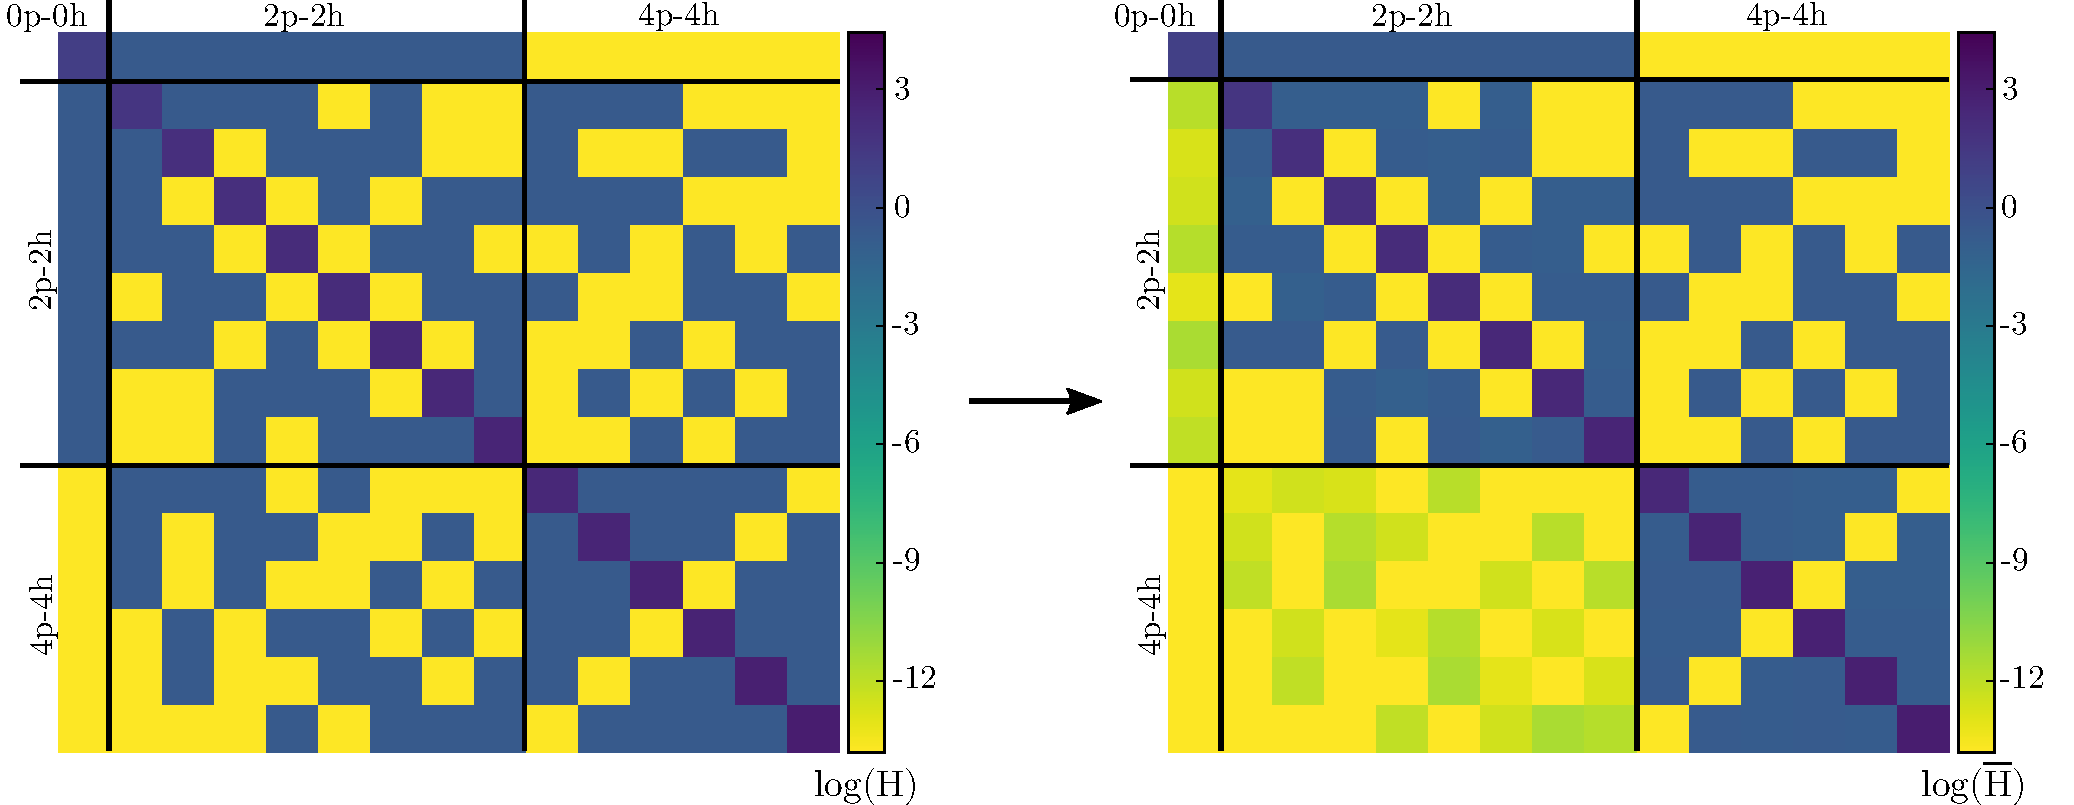
\includegraphics[width=\textwidth]{CC/pairingmatrix.pdf}
  \caption{ab-initio progress blah blah blah}
  \label{fig:pairingmatrix}
\end{figure}


\section{Example: Infinite Matter} \label{section:infinitematter}

Infinite nuclear or neutron matter is a homogeneous system and the one-particle wave functions are given by plane wave functions normalized to a volume $\Omega$ for a box with length $L$ (the limit $L\rightarrow \infty$ is to be taken after we have computed various expectation values)
\[
\psi_{\mathbf{k}\sigma}(\mathbf{r})=
\frac{1}{\sqrt{\Omega}}\exp{(i\mathbf{kr})}\xi_{\sigma}
\]
where $\mathbf{k}$ is the wave number and $\xi_{\sigma}$ is the spin
function for either spin up or down nucleons
\[ 
\xi_{\sigma=+1/2}=\left(\begin{array}{c} 1
  \\ 0 \end{array}\right) \hspace{0.5cm}
\xi_{\sigma=-1/2}=\left(\begin{array}{c} 0 \\ 1 \end{array}\right).
\]
As an interesting aside, the recent works of Binder {\em et al} \cite{binder2016} and McElvain and Haxton
\cite{haxton2016} offer new perspectives on the construction of effective Hamiltonians and choices of basis functions.


We focus first on the kinetic energy operator.  We assume that we have
periodic boundary conditions which limit the allowed wave numbers to
\[
k_i=\frac{2\pi n_i}{L}\hspace{0.5cm} i=x,y,z \hspace{0.5cm} n_i=0,\pm
1,\pm 2, \dots
\]
The operator for the kinetic energy can be written as
\[
\hat{T}=\sum_{\mathbf{p}\sigma_p}\frac{\hbar^2k_P^2}{2m}a_{\mathbf{p}\sigma_p}^{\dagger}a_{\mathbf{p}\sigma_p}.
\]
When using periodic boundary conditions, the discrete-momentum
single-particle basis functions (excluding spin and/or isospin degrees
of freedom) result in the following single-particle energy
\begin{align*}
  \varepsilon_{n_{x}, n_{y}, n_{z}} = \frac{\hbar^{2}}{2m} \left(
  \frac{2\pi }{L}\right)^{2} \left( n_{x}^{2} + n_{y}^{2} +
  n_{z}^{2}\right)=\frac{\hbar^2}{2m}\left(k_{n_x}^2+k_{n_y}^2+k_{n_z}^2\right),
\end{align*} 
for a three-dimensional system with
\[
k_{n_i}=\frac{2\pi n_i}{L}, \hspace{0.2cm} n_i = 0, \pm 1, \pm 2,
\dots,
\]
We will select the single-particle basis such that both the occupied
and unoccupied single-particle states have a closed-shell
structure. This means that all single-particle states corresponding to
energies below a chosen cutoff are included in the basis. We study
only the unpolarized spin phase, in which all orbitals are occupied
with one spin-up and one spin-down fermion (neutrons and protons in
our case).  With the kinetic energy rewritten in terms of the
discretized momenta we can set up a list (assuming
identical particles one and including spin up and spin down solutions)
of single-particle energies with momentum quantum numbers such that $n_{x}^{2}+n_{y}^{2}+n_{z}^{2}\le
3$, as shown in for example Table \ref{tab:table1}
\begin{table}
\begin{center}
\caption{Total number of particle filling $N_{\uparrow \downarrow }$
  for various $n_{x}^{2}+n_{y}^{2}+n_{z}^{2}$ values for one spin-1/2
  fermion species.  Borrowing from nuclear shell-model terminology,
  filled shells corresponds to all single-particle states for one
  $n_{x}^{2}+n_{y}^{2}+n_{z}^{2}$ value being occupied.  For matter
  with both protons and neutrons, the filling degree increased with a
  factor of $2$.} \label{tab:table1}
\begin{tabular}{ccccc}
\hline \multicolumn{1}{c}{ $n_{x}^{2}+n_{y}^{2}+n_{z}^{2}$ } &
\multicolumn{1}{c}{ $n_{x}$ } & \multicolumn{1}{c}{ $n_{y}$ } &
\multicolumn{1}{c}{ $n_{z}$ } & \multicolumn{1}{c}{ $N_{\uparrow
    \downarrow }$ } \\ \hline 0 & 0 & 0 & 0 & 2 \\ \hline 1 & -1 & 0 &
0 & \\ 1 & 1 & 0 & 0 & \\ 1 & 0 & -1 & 0 & \\ 1 & 0 & 1 & 0 & \\ 1 & 0
& 0 & -1 & \\ 1 & 0 & 0 & 1 & 14 \\ \hline 2 & -1 & -1 & 0 & \\ 2 & -1
& 1 & 0 & \\ 2 & 1 & -1 & 0 & \\ 2 & 1 & 1 & 0 & \\ 2 & -1 & 0 & -1 &
\\ 2 & -1 & 0 & 1 & \\ 2 & 1 & 0 & -1 & \\ 2 & 1 & 0 & 1 & \\ 2 & 0 &
-1 & -1 & \\ 2 & 0 & -1 & 1 & \\ 2 & 0 & 1 & -1 & \\ 2 & 0 & 1 & 1 &
38 \\ \hline 3 & -1 & -1 & -1 & \\ 3 & -1 & -1 & 1 & \\ 3 & -1 & 1 &
-1 & \\ 3 & -1 & 1 & 1 & \\ 3 & 1 & -1 & -1 & \\ 3 & 1 & -1 & 1 & \\ 3
& 1 & 1 & -1 & \\ 3 & 1 & 1 & 1 & 54 \\ \hline
\end{tabular}
\end{center}
\end{table}


Continuing in this way we get for $n_{x}^{2}+n_{y}^{2}+n_{z}^{2}=4$ a
total of 12 additional states, resulting in $66$ as a new magic
number. For the lowest six energy values the degeneracy in energy
gives us $2$, $14$, $38$, $54$, $66$ and $114$ as magic numbers. These
numbers will then define our Fermi level when we compute the energy in
a Cartesian basis. When performing calculations based on many-body
perturbation theory, coupled cluster theory or other many-body
methods, we need then to add states above the Fermi level in order to
sum over single-particle states which are not occupied.

If we wish to study infinite nuclear matter with both protons and
neutrons, the above magic numbers become $4, 28, 76, 108, 132, 228,
\dots$.

Every number of particles for filled shells defines also the number of
particles to be used in a given calculation. The number of particles
can in turn be used to define the density $\rho$ (or the Fermi momentum)
of the system via
\[
\rho = g \frac{k_F^3}{6\pi^2},
\]
where $k_F$ is the Fermi momentum and the degeneracy $g$, which is two
for one type of spin-$1/2$ particles and four for symmetric nuclear
matter.  With the density defined and having fixed the number of
particles $A$ and the Fermi momentum $k_F$, we can define the length
$L$ of the box used with periodic boundary contributions via the
relation
\[
  V= L^3= \frac{A}{\rho}.
\]
With $L$ we can to define the spacing between various
$k$-values given by
\[
  \Delta k = \frac{2\pi}{L}.
\]
Here, $A$ is the number of nucleons. If we deal with the electron
gas only, this needs to be replaced by the number of electrons $N$.
Exercise \ref{problem:spbasissetup} deals with the set up of a program
that establishes the single-particle basis for nuclear matter
calculations with input a given number of nucleons and a user
specificied density or Fermi momentum. 

\subsection{Two-body interaction\label{sec:interaction}}

As mentioned above, we will employ a plane wave basis for our
calculations of infinite matter properties. With a cartesian basis
we can calculate directly the various matrix elements. 
However, a cartesian basis
represents an approximation to the thermodynamical limit. In order to
compare the stability of our basis with results from the
thermodynamical limit, it is convenient to rewrite the nucleon-nucleon
interaction in terms of a partial wave expansion. This will allow us
to compute the Hartree-Fock energy of the ground state in the
thermodynamical limit (with the caveat that we need to limit the
number of partial waves). In order to find the expressions for the
Hartree-Fock energy in a partial wave basis, we will find it
convenient to rewrite our two-body force in terms of the relative and
center-of-mass motion momenta.

The direct matrix element, with single-particle three-dimensional
momenta $\mathbf{k}_p$, spin $\sigma_p$ and isospin $\tau_p$, is
defined as
\[
\langle \mathbf{k}_p\sigma_p\tau_p \mathbf{k}_q\sigma_q\tau_q \vert
\hat{v}\vert \mathbf{k}_r\sigma_r\tau_r \mathbf{k}_s\sigma_s\tau_s
\rangle,
\]
or in a more compact form as $\langle \mathbf{p}\mathbf{q}\vert
\hat{v} \vert \mathbf{r}\mathbf{s} \rangle$ where the boldfaced
letters $\mathbf{p}$ etc represent the relevant quantum numbers, here
momentum, spin and isospin. Introducing the relative momentum
\[
\mathbf{k} = \frac{1}{2}\left(\mathbf{k}_p-\mathbf{k}_q\right),
\]
and the center-of-mass momentum
\[
\mathbf{K} = \mathbf{k}_p+\mathbf{k}_q,
\]
we have
\[
\langle \mathbf{k}_p\sigma_p\tau_p \mathbf{k}_q\sigma_q\tau_q \vert
\hat{v}\vert \mathbf{k}_r\sigma_r\tau_r \mathbf{k}_s\sigma_s\tau_s
\rangle=\langle \mathbf{k}\mathbf{K}\sigma_p\tau_p \sigma_q\tau_q
\vert \hat{v}\vert \mathbf{k}'\mathbf{K}'\sigma_r\tau_r \sigma_s\tau_s
\rangle.
\]
The nucleon-nucleon interaction conserves the total momentum and
charge, implying that the above uncoupled matrix element reads
\[
\langle \mathbf{k}\mathbf{K}\sigma_p\tau_p \sigma_q\tau_q \vert
\hat{v}\vert \mathbf{k}'\mathbf{K}'\sigma_r\tau_r \sigma_s\tau_s
\rangle=\delta_{T_z,T_z'}\delta(\mathbf{K}-\mathbf{K}')\langle
\mathbf{k}T_zS_z=(\sigma_a+\sigma_b) \vert \hat{v}\vert
\mathbf{k}'T_zS_z'=(\sigma_c+\sigma_d) \rangle,
\]
where we have defined the isospin projections $T_z=\tau_p+\tau_q$ and
$T_z'=\tau_r+\tau_s$.  Defining
$\hat{v}=\hat{v}(\mathbf{k},\mathbf{k}' )$, we can rewrite the
previous equation in a more compact form as
\[
\delta_{T_z,T_z'}\delta(\mathbf{K}-\mathbf{K}')\langle
\mathbf{k}T_zS_z=(\sigma_p+\sigma_q) \vert \hat{v}\vert
\mathbf{k}'T_zS_z'=(\sigma_r+\sigma_s)
\rangle=\delta_{T_z,T_z'}\delta(\mathbf{K}-\mathbf{K}')\langle
T_zS_z\vert\hat{v}(\mathbf{k},\mathbf{k}' ) \vert T_zS_z' \rangle.
\]
These matrix elements can in turn be rewritten in terms of the total
two-body quantum numbers for the spin $S$ of two spin-1/2 fermions as
\[
\langle \mathbf{k}T_zS_z \vert \hat{v}(\mathbf{k},\mathbf{k}' )\vert
\mathbf{k}'T_zS_z' \rangle=\sum_{SS'}\langle
\frac{1}{2}\sigma_p\frac{1}{2}\sigma_q\vert SS_z\rangle \langle
\frac{1}{2}\sigma_r\frac{1}{2}\sigma_s\vert S'S_z'\rangle \langle
\mathbf{k}T_zSS_z\vert \hat{v}(\mathbf{k},\mathbf{k}' )\vert
\mathbf{k}T_zS'S_z' \rangle
\]
The coefficients $\langle \frac{1}{2}\sigma_p\frac{1}{2}\sigma_q\vert
SS_z\rangle$ are so-called Clebsch-Gordan recoupling coefficients.  We
will assume that our interactions conserve charge. We will refer to $T_z=0$ as the $pn$ (proton-neutron)
channel, $T_z=-1$ as the $pp$ (proton-proton) channel and $T_z=1$ as
the $nn$ (neutron-neutron) channel.

The nucleon-nucleon force is often derived and analyzed theoretically
in terms of a partial wave expansion. A state with linear momentum
$\mathbf{k}$ can be written in terms of spherical harmonics $Y_{lm}$ as
\[
\vert \mathbf{k} \rangle =
\sum_{l=0}^{\infty}\sum_{m=-l}^{l}\imath^lY_{lm}\langle\hat{k}\vert
klm_l\rangle.
\]

In terms of the relative and center-of-mass momenta $\mathbf{k}$ and
$\mathbf{K}$, the potential in momentum space is related to the
nonlocal operator $V(\mathbf{r},\mathbf{r}')$ by
\begin{equation*}
      \langle \mathbf{k'K'}\vert \hat{v} \vert \mathbf{k'K} \rangle=
      \int d\mathbf{r}d \mathbf{r'} e^{-\imath
        \mathbf{k'r'}}V(\mathbf{r'},\mathbf{r}) e^{\imath \mathbf{kr}}
      \delta(\mathbf{K},\mathbf{K'}).
\end{equation*}
We will assume that the interaction is spherically symmetric and use
the partial wave expansion of the plane waves in terms of spherical
harmonics.  This means that we can separate the radial part of the
wave function from its angular dependence. The wave function of the
relative motion is described in terms of plane waves as
\begin{equation*}
       e^{\imath \mathbf{kr}} = \langle\mathbf{r}\vert
       \mathbf{k}\rangle = 4\pi \sum_{lm} \imath ^{l} j_{l} (kr)
       Y_{lm}^{*}(\mathbf{\hat{k}}) Y_{lm}(\mathbf{\hat{r}}),
\end{equation*}
where $j_l$ is a spherical Bessel function and $Y_{lm}$ the spherical
harmonic.  This partial wave basis is useful for defining the operator
for the nucleon-nucleon interaction, which is symmetric with respect
to rotations, parity and isospin transformations. These symmetries
imply that the interaction is diagonal with respect to the quantum
numbers of total angular momentum $J$, spin $S$ and isospin $T$. Using
the above plane wave expansion, and coupling to final $J$, $S$ and $T$
we get
\begin{equation*}
      \langle \mathbf{k'}\vert V \vert \mathbf{k}\rangle = (4\pi)^2
      \sum_{JM}\sum_{lm}\sum_{l'm'} \imath ^{l+l'}
      Y_{lm}^{*}(\mathbf{\hat{k}}) Y_{l'm'}(\mathbf{\hat{k}'}) {\cal
        C}_{m'M_SM}^{l'SJ}{\cal C}_{mM_SM}^{lSJ} \langle k'l'STJM
      \vert V \vert klSTJM \rangle,
\end{equation*}
where we have defined
\begin{equation*}
    \langle k'l'STJM\vert V \vert klSTJM\rangle = \int
    j_{l'}(k'r')\langle l'STJM\vert V(r',r)\vert lSTJM \rangle j_l(kr)
    {r'}^2 dr' r^2 dr.
\end{equation*}
We have omitted the momentum of the center-of-mass motion $\mathbf{K}$
and the corresponding orbital momentum $L$, since the interaction is
diagonal in these variables. 

The interaction we will use for these calculations is a semirealistic
nucleon-nucleon potential known as the Minnesota potential
\cite{minnesota} which has the form, $V_{\alpha}\left(
r\right)=V_{\alpha}\exp{(-\alpha r^{2})}$. The spin and isospin
dependence of the Minnesota potential is given by,
\begin{equation*}
V\left( r\right)=\frac{1}{2}\left( V_{R}+\frac{1}{2}\left(
1+P_{12}^{\sigma}\right) V_{T}+\frac{1}{2}\left(
1-P_{12}^{\sigma}\right) V_{S}\right)\left(
1-P_{12}^{\sigma}P_{12}^{\tau}\right),
\end{equation*}
where $P_{12}^{\sigma}=\frac{1}{2}\left(
1+\sigma_{1}\cdot\sigma_{2}\right)$ and
$P_{12}^{\tau}=\frac{1}{2}\left( 1+\tau_{1}\cdot\tau_{2}\right)$ are
the spin and isospin exchange operators, respectively. A Fourier
transform to momentum space of the radial part $V_{\alpha}\left(
r\right)$ is rather simple, see problem \ref{problem:fourier}, since
the radial depends only on the magnitude of the relative distance and
thereby the relative momentum
$\vec{q}=\frac{1}{2}\left(\vec{k}_{p}-\vec{k}_{q}-\vec{k}_{r}+\vec{k}_{s}\right)$. Omitting
spin and isospin dependencies, the momentum space version of the
interaction reads
\begin{equation*}
\langle \mathbf{k}_p \mathbf{k}_q \vert V_{\alpha}\vert
\mathbf{k}_r\mathbf{k}_s\rangle=\frac{V_{\alpha}}{L^{3}}\left(\frac{\pi}{\alpha}\right)^{3/2}\exp{(\frac{-q^{2}}{4\alpha})}\delta_{\vec{k}_{p}+\vec{k}_{q},\vec{k}_{r}+\vec{k}_{s}}
\end{equation*}
The various parameters defining the interaction model used in this
work are listed in Table \ref{tab:minnesotatab}.
\begin{table}
\caption{Parameters used to define the Minnesota interaction model
  \cite{minnesota}.}\label{tab:minnesotatab}
\begin{center}
  \begin{tabular}{| l | l | l |}
    \hline $\alpha$ & $V_{\alpha}$ in $\mathrm{MeV}$ & $\kappa_{\alpha}$ in $\mathrm{fm}^{-2}$  \\ \hline $R$ &
    200  & 1.487 \\ \hline $T$ & 178
     & 0.639 \\ \hline $S$ & 91.85
    & 0.465  \\ \hline
  \end{tabular}
\end{center}
\end{table}

In these calculations we
approximated our problem with periodic boundary conditions,
  $\mathop{\phi(x_{i})}=\mathop{\phi(x_{i}+L)}$, but we could have
  chosen anti-periodic boundary conditions,
  $\mathop{\phi(x_{i})}=-\mathop{\phi(x_{i}+L)}$. The difference
  between these two shows how the correlation energy contains
  finite-size effects \cite{gros1992,gros1996,shepherd2012,shepherd2016}. One solution to this problem is by integrating
  over solutions between periodic and anti-periodic conditions, known
  as twist-averaging \cite{twistaverage}. First, we multiply the single-particle states by
  a phase for each direction, characterized by a twist-angle,
  $\theta_{i}$.
  \begin{equation}
    \mathop{\phi_{\vec{k}}(\vec{x}+\vec{L})}\rightarrow\mathop{e^{i\vec{\theta}}\phi_{\vec{k}}(\vec{x})}
  \end{equation}
  $\theta_{i}=0$ for PBC and $\theta_{i}=\pi$ for APBC
  \begin{align}
  \vec{k}\rightarrow\vec{k}+\frac{\vec{\theta}}{L}
  \\ \epsilon_{\vec{k}}\rightarrow\epsilon_{\vec{k}}+\frac{\pi}{L}\vec{k}\cdot\vec{\theta}+\frac{\pi^{2}}{L^{2}}
  \end{align}
  Adding these phases changes the single-particle energies, the
  correction of which disappear as $L\rightarrow\infty$, depending on
  $\vec{\theta}$ and thus changes the shell structure so that hole
  states can jump up to particle states and {\em vice versa}. It is thence
  necessary to fill hole states separately for each
  $\vec{\theta}$. Integration over a quantitiy is approximated by a
  weighted sum, such as Gauss-Legendre quadrature, over the quantity
  for each set of twist angles. The algorithm becomes then
\begin{svgraybox}
  \begin{algorithmic}
    \State Build mesh points and weights for each direction $i$:
    $\{\theta_{i},w_{i}\}$ \State $E_{\text{twist}}=0$
    \For{$\mathop{(\theta_{x},w_{x})}\in\mathop{\{\theta_{x},w_{x}\}}$}
    \For{$\mathop{(\theta_{y},w_{y})}\in\mathop{\{\theta_{y},w_{y}\}}$}
    \For{$\mathop{(\theta_{z},w_{z})}\in\mathop{\{\theta_{z},w_{z}\}}$}
    \State Build Basis States with $k_{i}\rightarrow
    k_{i}+\frac{\theta_{i}}{L}$ \State Order States by Energy and Fill
    Holes \State Get Result $E$ (T,HF,CCD) \State
    $E_{\text{twist}}=E_{\text{twist}}+\frac{1}{\pi^{3}}w_{x}w_{y}w_{z}E$
    \EndFor \EndFor \EndFor
  \end{algorithmic}
\end{svgraybox}
  This technique gives results which depend much less on the particle
  number, but requires a full calculation for each set of twist
  angles, which can grow very quickly. For example, using 10 twist
  angles in each direction requires 1000 calculations. To see the
  effects of twist averaging, it is easy to calculate the kinetic
  energy per particle and the Hartree-Fock energy per particle, which
  avoids the full CCD calculation. These calculations can be compared
  to the exact values for infinite matter, which are calculated by
  integrating the the relevent values up to the fermi surface. The kinetic energy is given by
  \[
\text{T}_{\text{inf}}=\frac{3\hbar^{2}k_{f}^{2}}{10m},
\]
while the potential energy to first order (corresponding to the Hartree-Fock contribution) reads
\[
\text{HF}_{\text{inf}}=\frac{1}{\mathop{(2\pi)^{6}}}\frac{L^{3}}{2\rho}\int_{0}^{k_{f}}d\vec{k}_{1}\int_{0}^{k_{f}}d\vec{k}_{2}\braket{\vec{k}_{1}\vec{k}_{2}|\hat{v}|\vec{k}_{1}\vec{k}_{2}}.
\]
Figure \ref{fig:fig3} shows the CCD kinetic energy of pure neutron
      matter computed with the Minnesota interaction model  \cite{minnesota} as a function of
      the number of particles for both periodic boundary conditions (PBC)
      and twist-averaged boundary conditions (TABC5). We see clearly that the 
twist-averaged boundary conditions soften the dependence on finite size effects. 
  \begin{figure}
    \includegraphics[width=\linewidth]{Chapter8-figures/fig3.pdf}
    \caption{Finite-size effects in the kinetic energy of pure neutron
      matter computed with the Minnesota interaction model  \cite{minnesota} as a function of
      the number of particles for both periodic boundary conditions (PBC)
      and twist-averaged boundary conditions (TABC5).}
    \label{fig:fig3}
  \end{figure}
Similarly, Fig.~\ref{fig:fig4} displays the corresponding Hartree-Fock energy (the reference energy) 
obtained with Minnesota interaction using both periodic and twist-average boundary conditions.  
  \begin{figure}
    \includegraphics[width=\linewidth]{Chapter8-figures/fig4.pdf}
    \caption{Finite-size effects in the Hartree-Fock energy of pure
      neutron matter computed with the Minnesota interaction model  \cite{minnesota} as a
      function of the number of particles for both periodic boundary (PBC)
      conditions and twist-averaged boundary conditions (TABC5).}
    \label{fig:fig4}
  \end{figure}
The results show again a weaker dependence on finite size effects.

With all these ingredients, we can now compute the final CCD energy and thereby the equation of state for infinite neutron matter.
Figure \ref{fig:finalccdenergy} displays the total CCD energy (including the reference energy) as well as the reference energy
obtained with the Minnesota interaction model. The computations have been performed with $N=66$ neutrons and a maximum number of single-particle states constrained by $N_{max}=36$. This corresponds to $2377$ single-particle states. 
  \begin{figure}
    \includegraphics[width=\linewidth]{Chapter8-figures/finalccenergy.pdf}
    \caption{Energy per particle for pure neutron matter as function of density from coupled cluster calculations with doubles correlations  only. The reference energy is included for comparison. The results have been obtained with Minnesota interaction model using periodic  boundary conditions and $N=66$ neutrons and single-particle states up to $N_{max}=36$, resulting in a total of $2377$ single-particle states. }  
    \label{fig:finalccdenergy}
  \end{figure}
We see from this figure that the correlations brought by coupled cluster theory are at the order of $10\%$ roughly of the reference energy. It means that for this system (neutrons only) with the Minnesota potential, higher-order correlations can most likely be treated in a perturbative way. Many-body perturbation theory to second order gives results which are very close to our CCD results, as seen in 
Table \ref{tab:ecomparison}.
\begin{table}
\caption{CCD and MBPT2 results for infinite neutron matter with $N=66$ neutrons and a maximum number of single-particle states constrained by $N_{max}=36$. }\label{tab:ecomparison}
  \begin{center}
      \begin{tabular}{| l | l | l |}
      \hline Density $\rho$ fm$^{-3}$ & $E_{MBPT2}$ & $E_{CCD}$
      \\ \hline 0.04 & 6.472   & 6.468    \\ \hline
      0.06 & 7.919  & 7.932   \\ \hline
      0.08 & 9.075  & 9.136    \\ \hline
      1.0 & 9.577 &  10.074  \\  \hline
      1.2 & 10.430 & 10.885   \\ \hline
      1.4 & 11.212 & 11.565   \\  \hline
      1.6 & 11.853  & 12.136    \\  \hline
      1.8 & 12.377 & 12.612   \\ \hline
      2.0 & 12.799 & 13.004   \\ \hline
      \end{tabular}
  \end{center}
\end{table}
For low densities we observe a good agreement while higher densities
bring in particle-particle correlations that become more important as
the density increases. Coupled cluster theory sums to infinite order for
example particle-particle correlations and with increasing densities
this is reflected in differences between the two many-body
approximations.  The above results agree well with the recent coupled
cluster calculations of Refs.~\cite{baardsen2013,hagenmatter}, obtained with
interaction models from effective field theory.  With the inclusion of
proton correlations as well as other potential models we may expect 
larger differences between
different methods and interactions.  In chapters 9, 10 and 11 we compare the above results with 
those obtained with Monte Carlo methods, the in-medium renormalization group approach and Green's function theory.


\end{document}
